\section{Ristoratore}
\label{cap:amministrazione}
\subsection{Area Privata}
L'\emph{My Area} (Figura~\ref{fig:myarea-owner}) offre:
\begin{itemize}
    \item Elenco dei ristoranti gestiti e relative recensioni.
    \item Pulsante “\texttt{Add Restaurant}” per l'inserimento di nuove attività.
    \item Elenco delle recensioni lasciate ad altri ristoranti.
\end{itemize}

\begin{figure}[H]
    \centering
    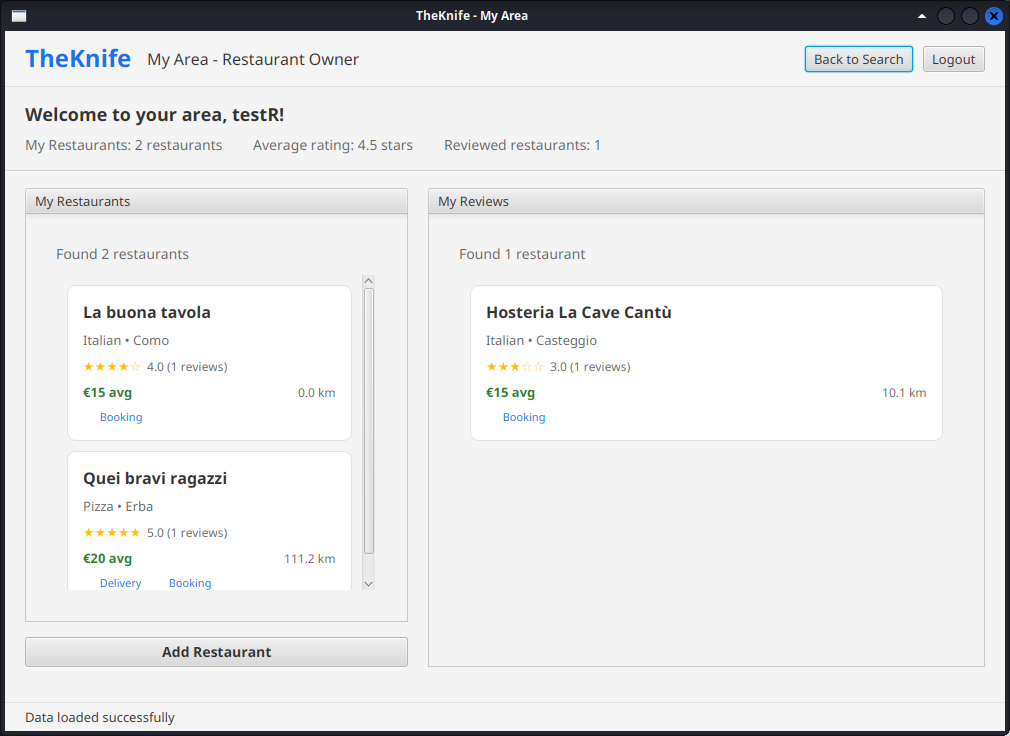
\includegraphics[width=0.8\textwidth]{images/myarea-owner.png}
    \caption{Schermata Area Privata Ristoratore}
    \label{fig:myarea-owner}
\end{figure}

\subsection{Creazione ristorante}
Per aggiungere un nuovo ristorante, premere il pulsante \emph{Add Restaurant} (Figura~\ref{fig:add-restaurant}) e compilare tutti i campi.
\begin{figure}[H]
    \centering
    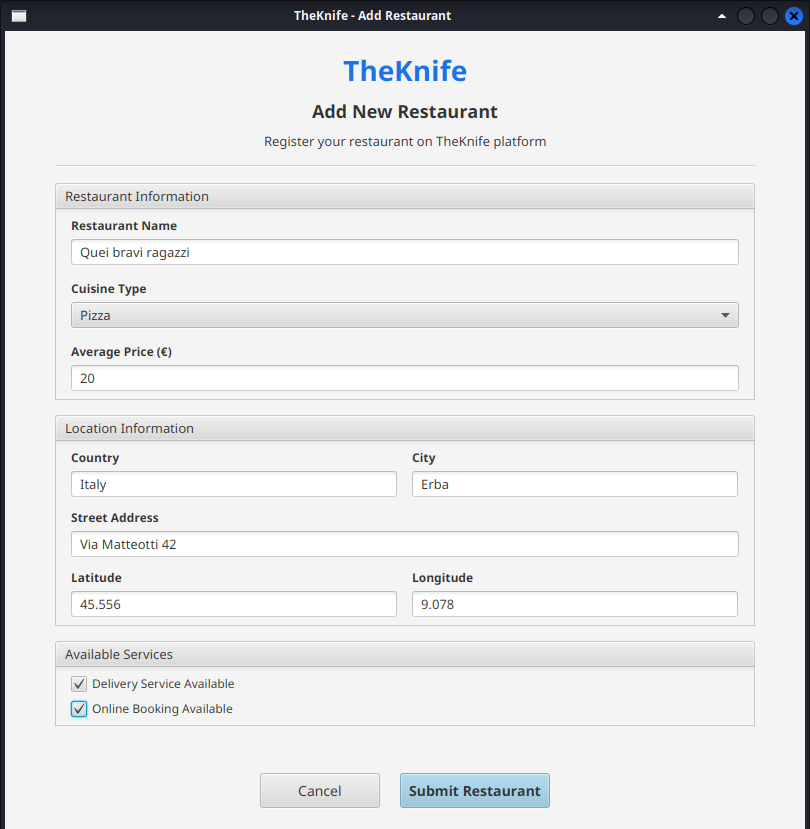
\includegraphics[width=0.8\textwidth]{images/add-restaurant.png}
    \caption{Interfaccia per la creazione di un ristorante}
    \label{fig:add-restaurant}
\end{figure}

\subsection{Risposte alle recensioni}
I proprietari possono rispondere (Figura~\ref{fig:reply}) alle recensioni dei propri locali premendo 
sulla recensinoe desiderata nell'elenco delle recensioni ricevute.
\begin{figure}[H]
    \centering
    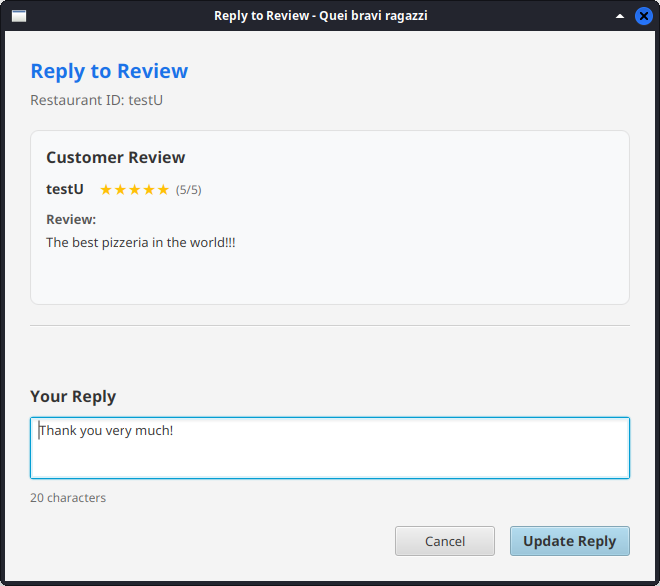
\includegraphics[width=0.8\textwidth]{images/reply.png}
    \caption{Interfaccia per la gestione delle risposte}
    \label{fig:reply}
\end{figure}
